\chapter{Results}
\label{ch:results}

\section{Simulations and Uncertainties}

\subsection{Simulations on Global Properties}
Interpretation of Global Fractal Dimension
Scale-free GRF vs GRF with Scale

\subsection{Simulations on Local Properties}

\subsection{Error Estimates}

The uncertainties on the perimeter and area measurements, estimated using the simulation procedures described above, are on average approximately 1.60\% for each quantity. These uncertainties arise primarily from pixelation effects and resolution limitations in the column density maps.  

An example of the resulting error distributions from a representative simulation run is shown in Figure~\ref{fig:uncertainties}. The narrow spread around the mean confirms that the estimates are robust and systematic errors remain small compared to the dynamic range of the measurements.

\begin{figure}[t]
    \centering
    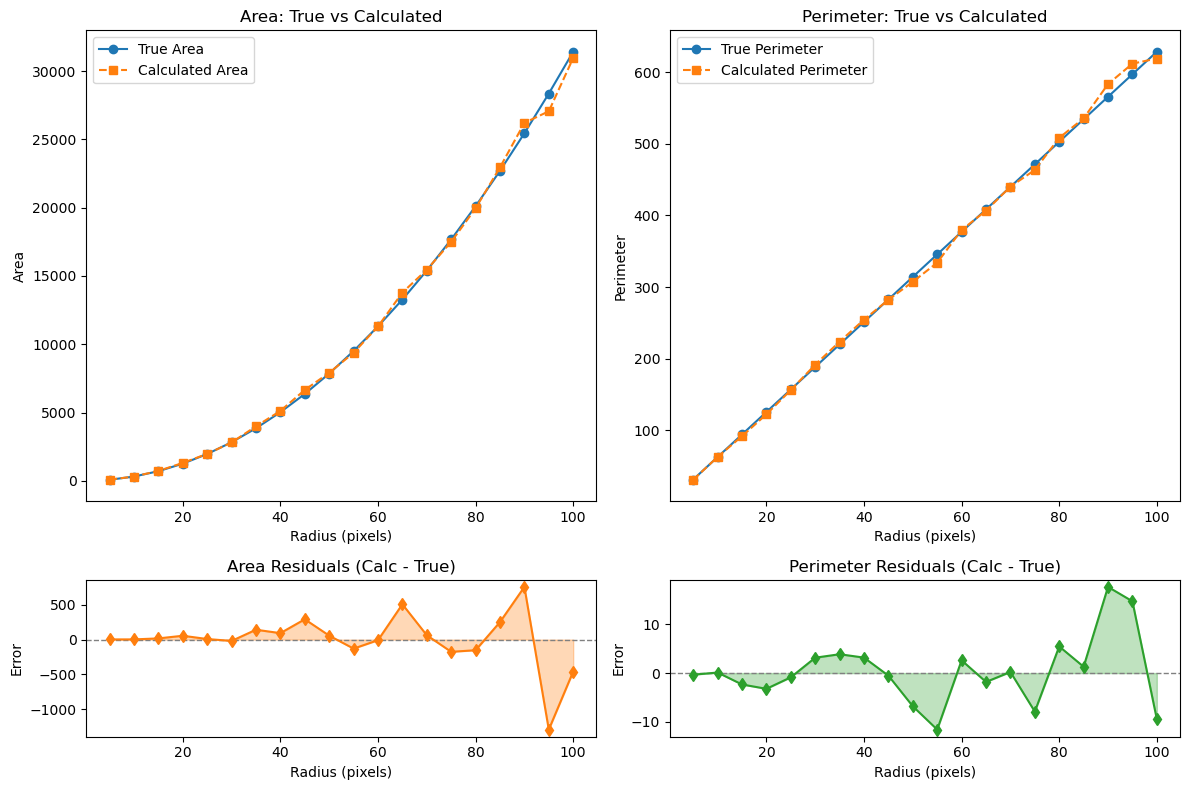
\includegraphics[width=0.75\textwidth]{figures/perimeter_area_uncertainties.png}
    \caption{Example of the uncertainty distributions in the measurements of perimeter and area from simulated structures (arbitrary units).}
    \label{fig:uncertainties}
\end{figure}

\section{Global Properties}

% Uncertainties
\subsection{Global Fractal Dimension}

The perimeter and area measurements are computed over a restricted range of column densities, specifically between $N_\mathrm{min}$ and $N_\mathrm{max}$. This selection is made to avoid biases introduced by the limited resolution and artificially straight contours that occur at low column densities, as well as the small number of pixels and irregular shapes that dominate at very high column densities.

Figure \ref{fig:orion_A_global} shows the perimeter-area relation for Orion A, along with the best-fit linear regression used to derive the global fractal dimension. The resulting estimate, including the uncertainty from the fit, is:

\begin{equation}
    \notag
    D_{\mathrm{OA,\,Global}} = 1.35 \pm 0.02
\end{equation}

\begin{figure}[t]
    \centering
    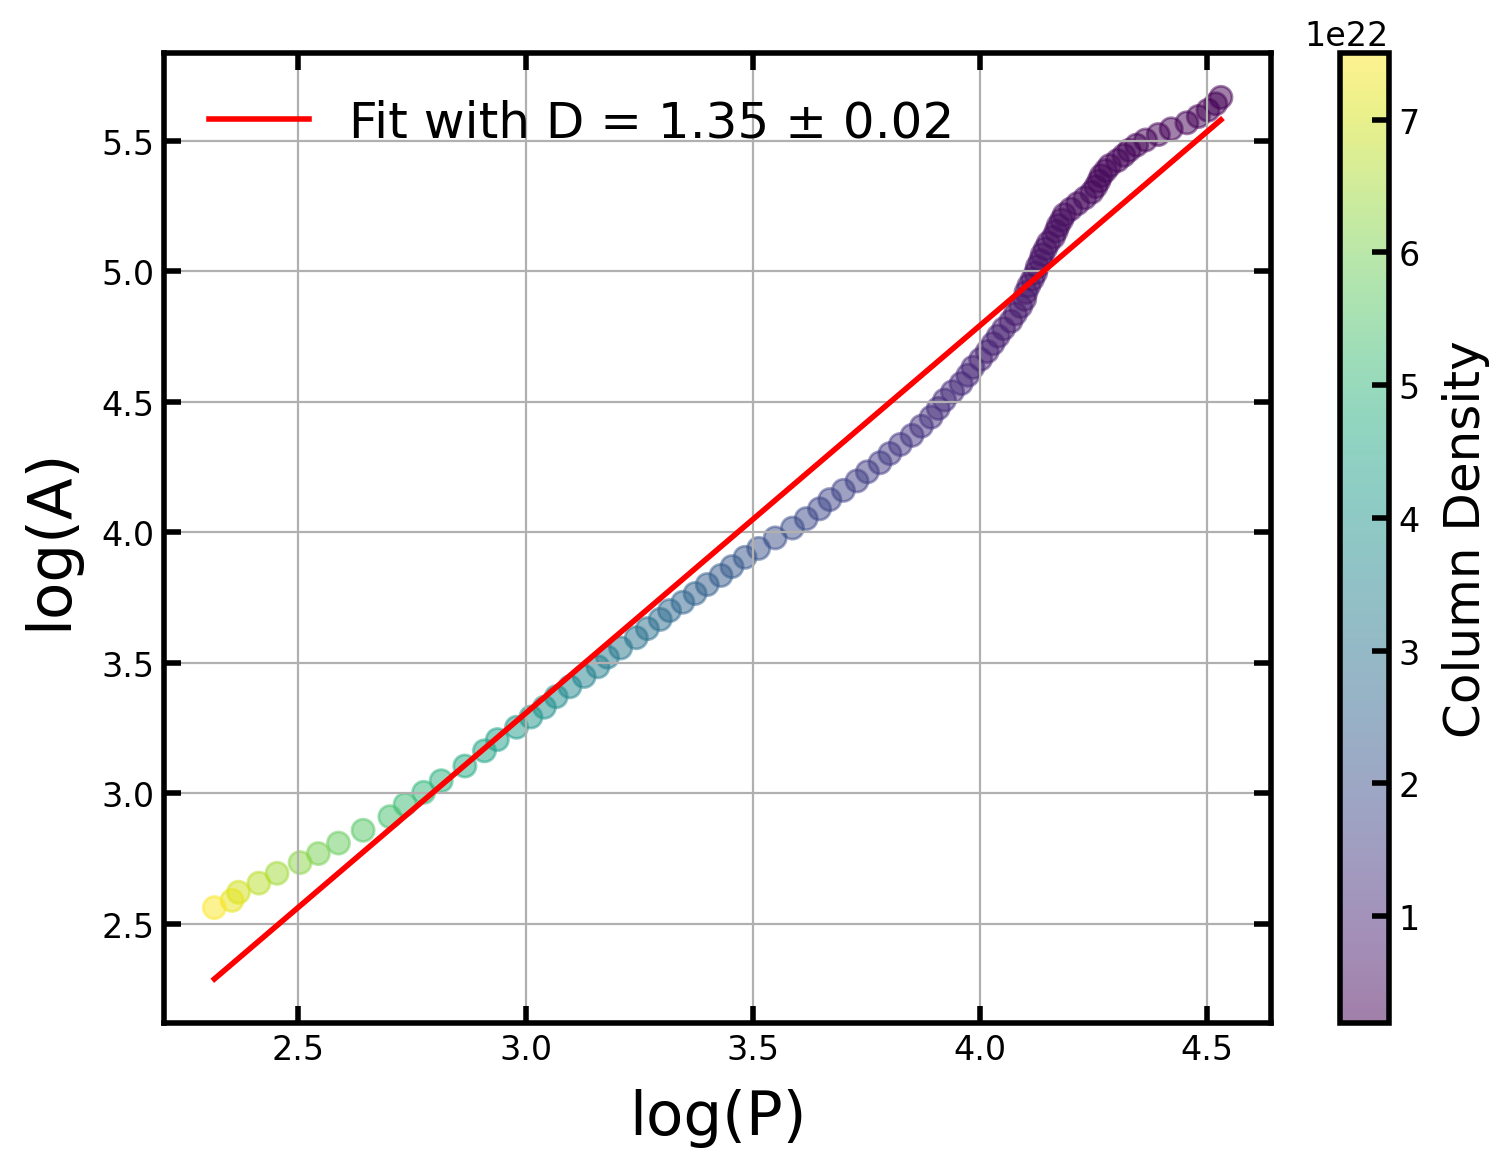
\includegraphics[width=0.75\textwidth]{figures/orion_A_global.png}
    \caption{Perimeter-area relation for Orion A. The dashed line shows the linear fit in log--log space used to estimate the global fractal dimension $D$. Residuals of the fit are shown below the main panel.}
    \label{fig:orion_A_global}
\end{figure}

The Orion A cloud exhibits significant deviations from a single linear fit over the entire column density range. To account for this, a segmented (double) linear fit was applied, splitting the data at $N = 1.23 \times 10^{22}\,\mathrm{cm}^{-2}$. The results of the two fits are:

\begin{equation}
    \notag
    D_1 = 1.65 \pm 0.01 \quad \text{(low column density)}
\end{equation}
\begin{equation}
    \notag
    D_2 = 0.97 \pm 0.02 \quad \text{(high column density)}
\end{equation}

Figure \ref{fig:orion_A_global_double_fit} shows the perimeter--area relation with the two linear fits overlaid. The change in slope suggests a structural transition or the presence of different regimes of spatial complexity in the cloud.
% switch low and high
\begin{figure}[t]
    \centering
    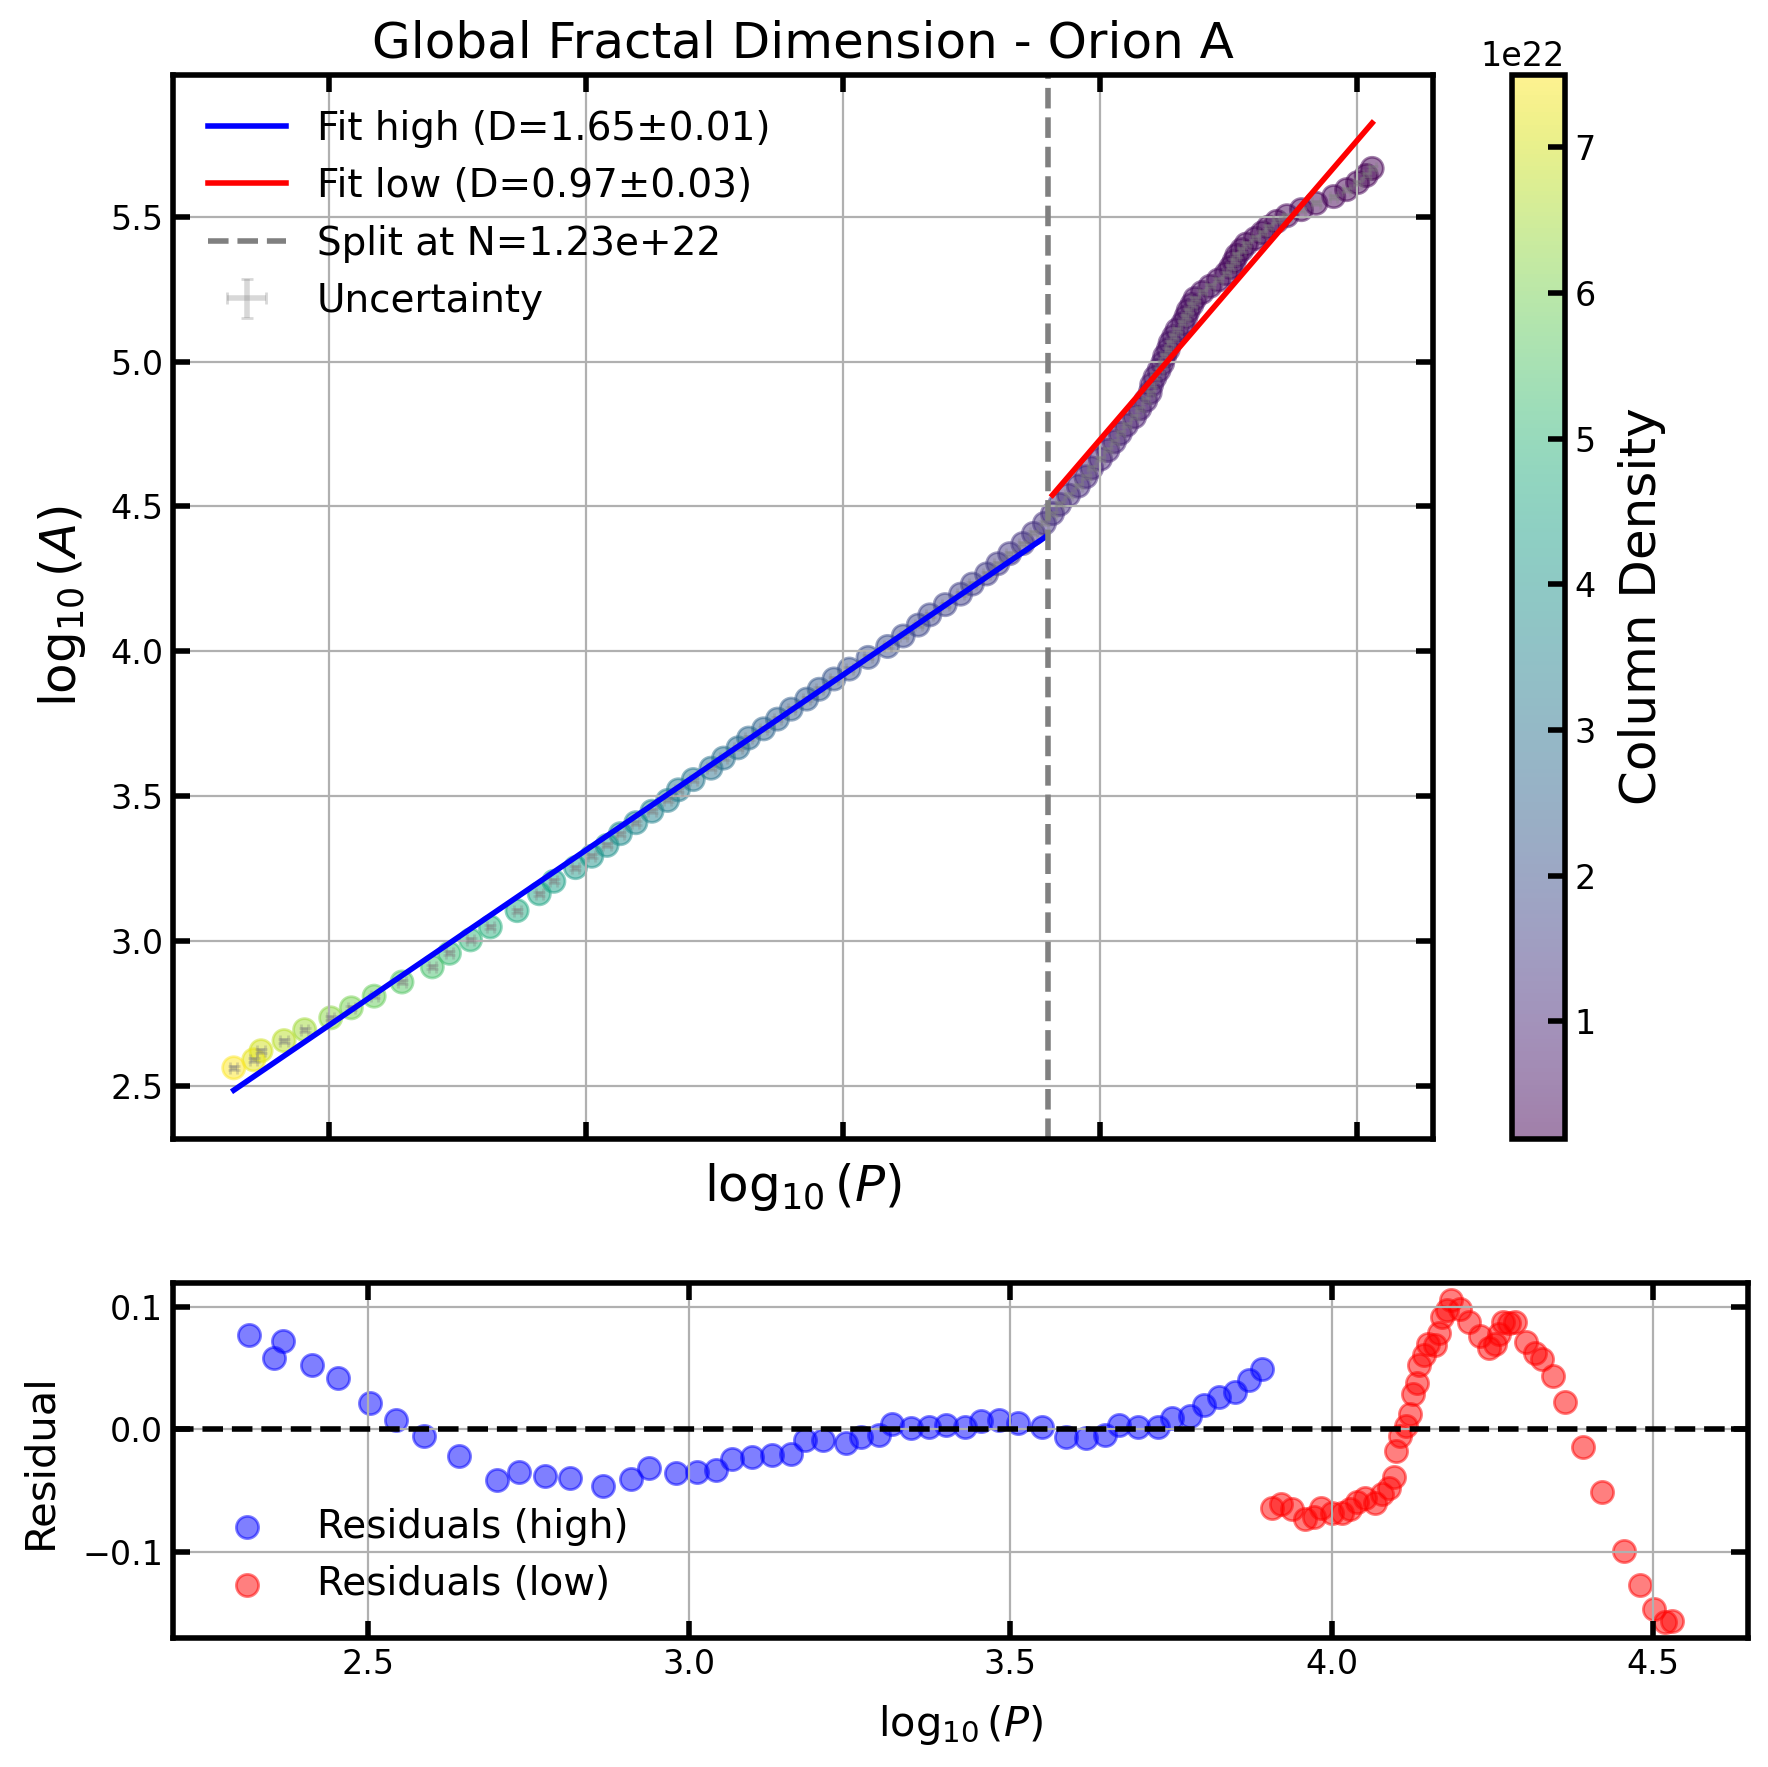
\includegraphics[width=0.75\textwidth]{figures/orion_A_global_double_fit.png}
    \caption{Perimeter-area relation for Orion A with a segmented (double) linear fit. The dashed lines indicate the two fitted regimes, separated at $N=1.23 \times 10^{22}\,\mathrm{cm}^{-2}$.}
    \label{fig:orion_A_global_double_fit}
\end{figure}

The Orion B cloud exhibits a well-behaved perimeter-area relation that can be accurately described by a single linear fit across the entire column density range. The results are:

\begin{equation}
    \notag
    D_{\mathrm{OB,\,Global}} = 1.40 \pm 0.01
\end{equation}

Figure \ref{fig:orion_B_global} shows the perimeter-area relation together with the fitted line. The consistency of the slope across scales suggests a more uniform structural complexity compared to Orion A.

\begin{figure}[t]
    \centering
    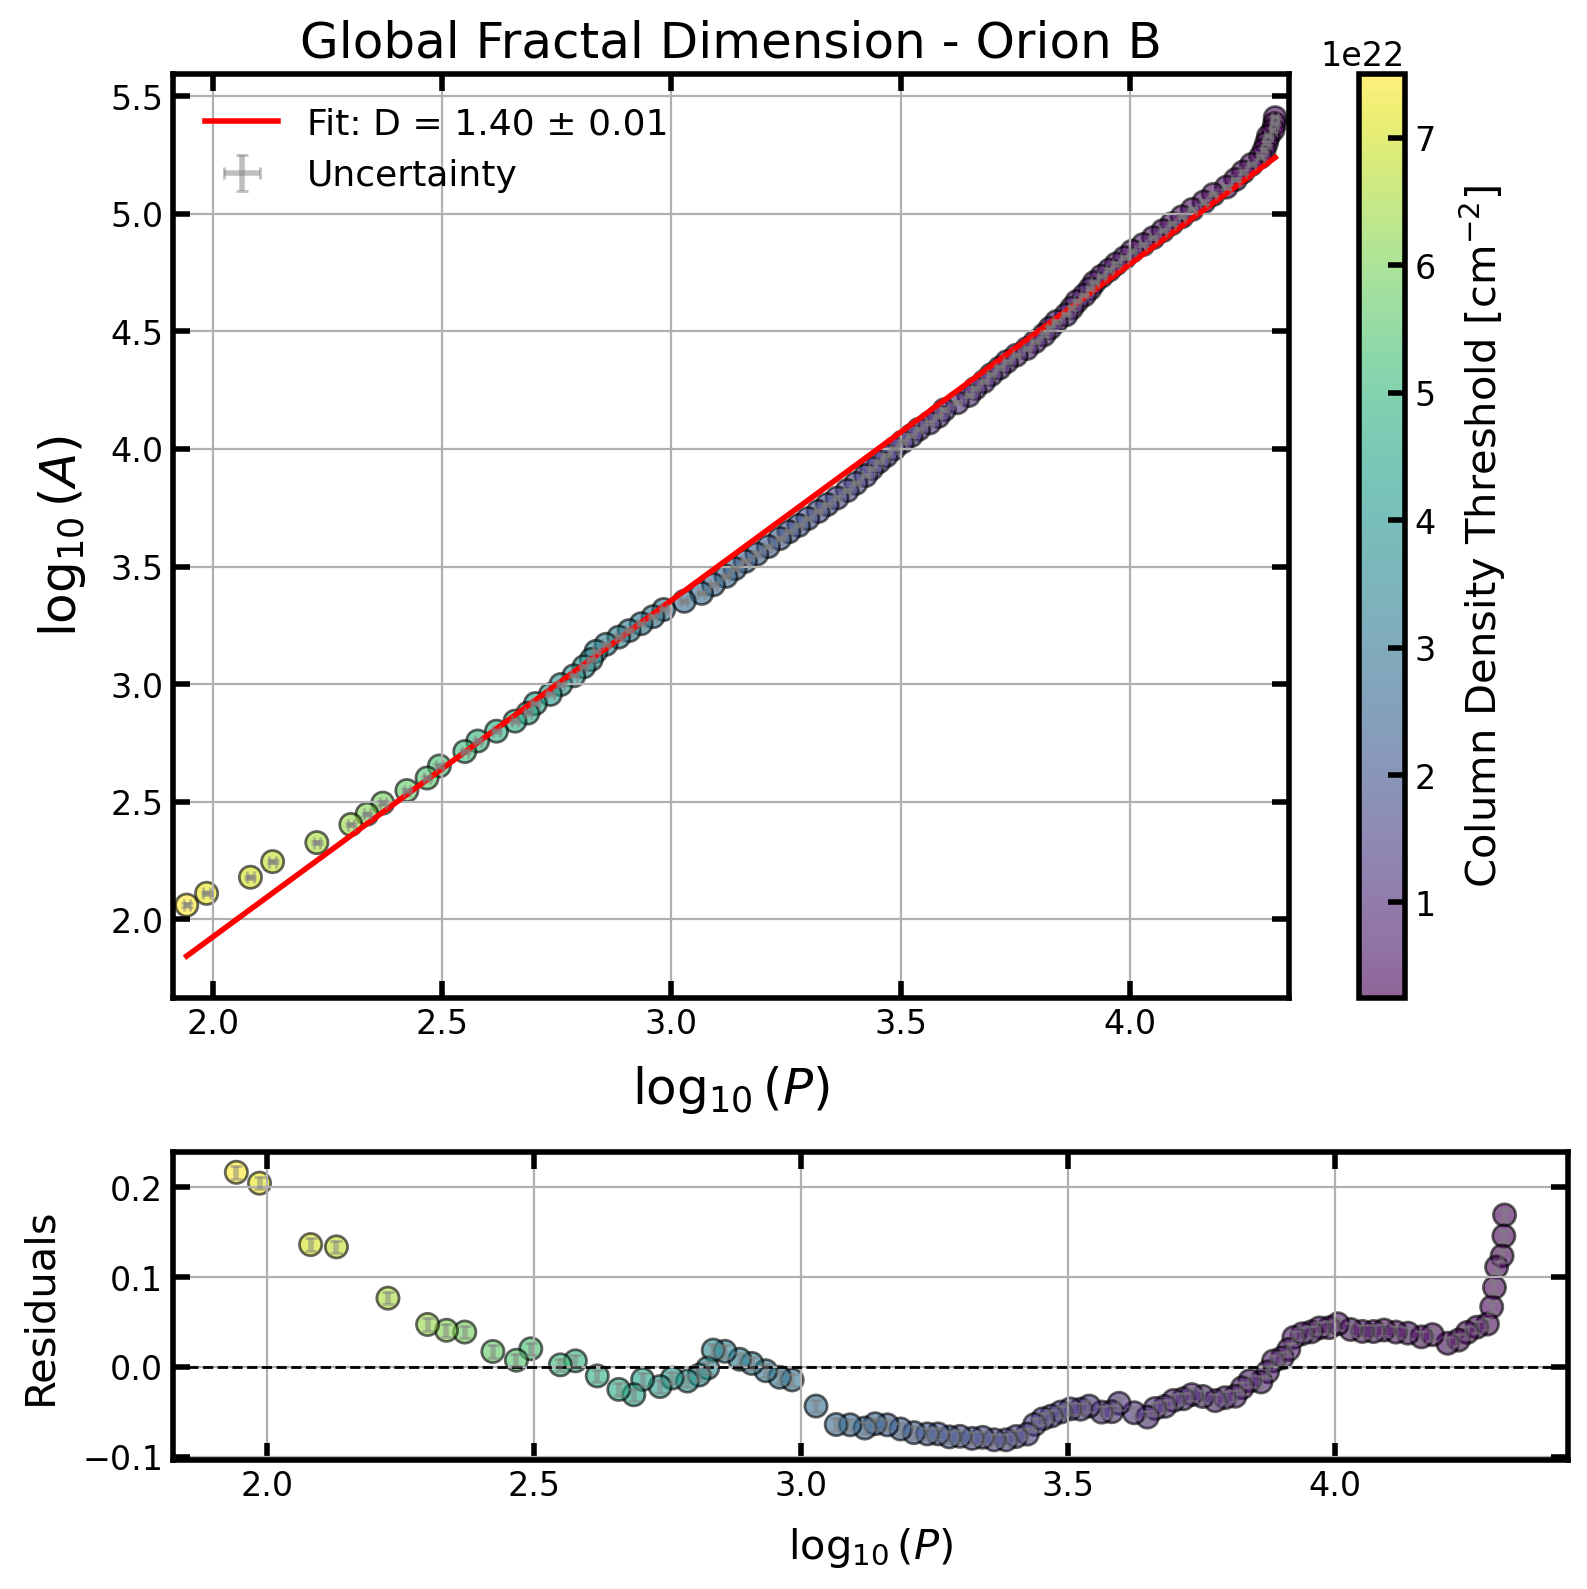
\includegraphics[width=0.75\textwidth]{figures/orion_B_global.png}
    \caption{Perimeter-area relation for Orion B with the best-fit linear regression overlaid.}
    \label{fig:orion_B_global}
\end{figure}

ADD: The uncertainty from P and A are taken to be 1.6\% via the 
The uncertainties are calculated from the fit routine, since the 

\section{Local Properties}

\subsection{Local Fractal Dimension}

Data Orion A and Orion B

Single structures

\begin{figure}[t]
    \centering
    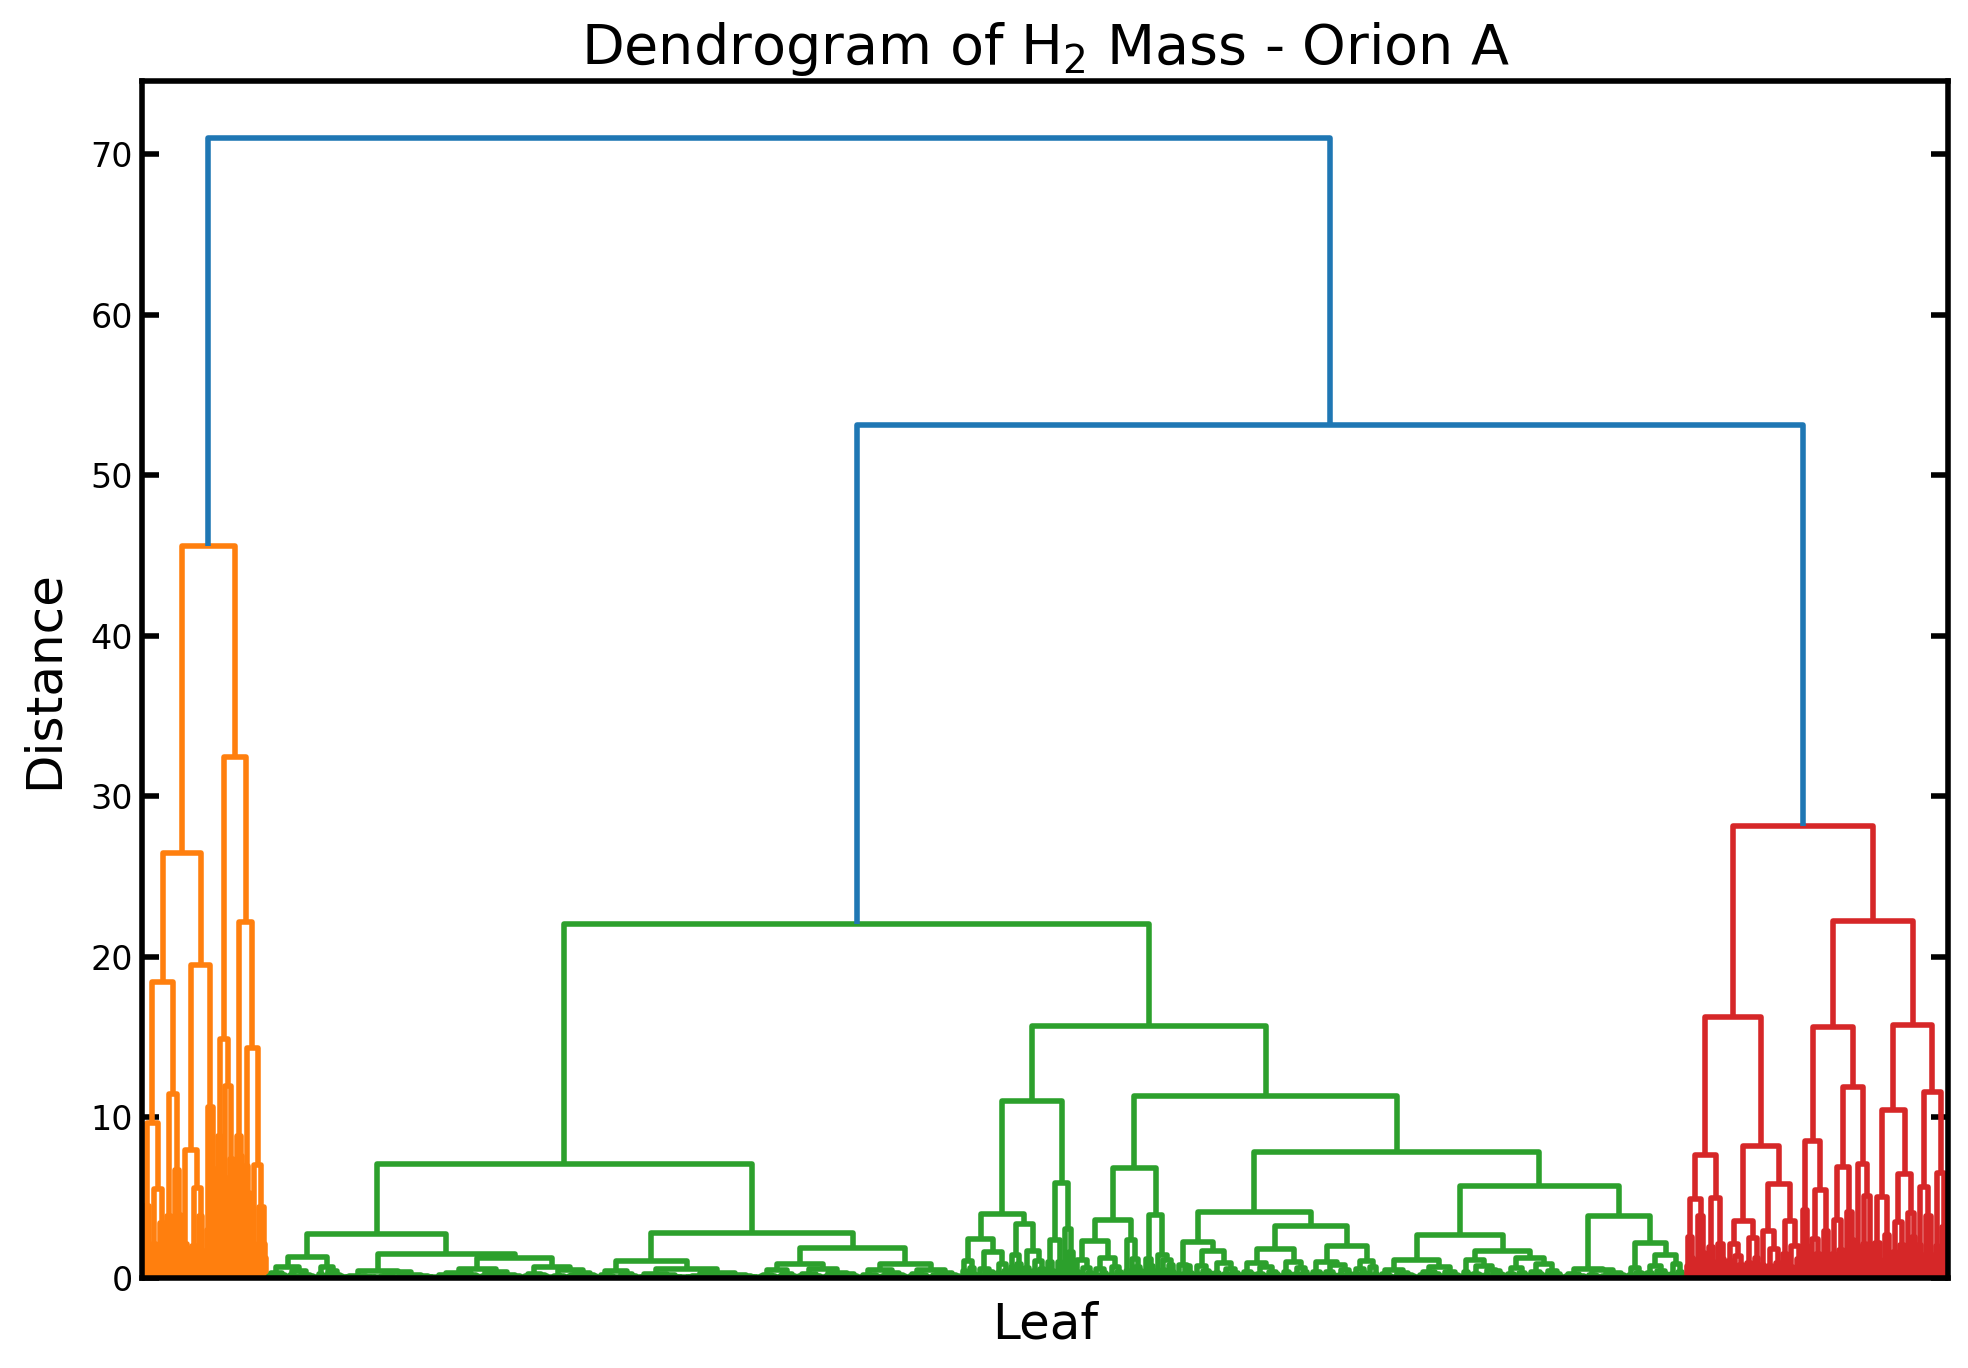
\includegraphics[width=0.5\textwidth]{figures/dendogram_A.png}
    \caption{}
    \label{fig:dendrogram_A}
\end{figure}

\begin{figure}[t]
    \centering
    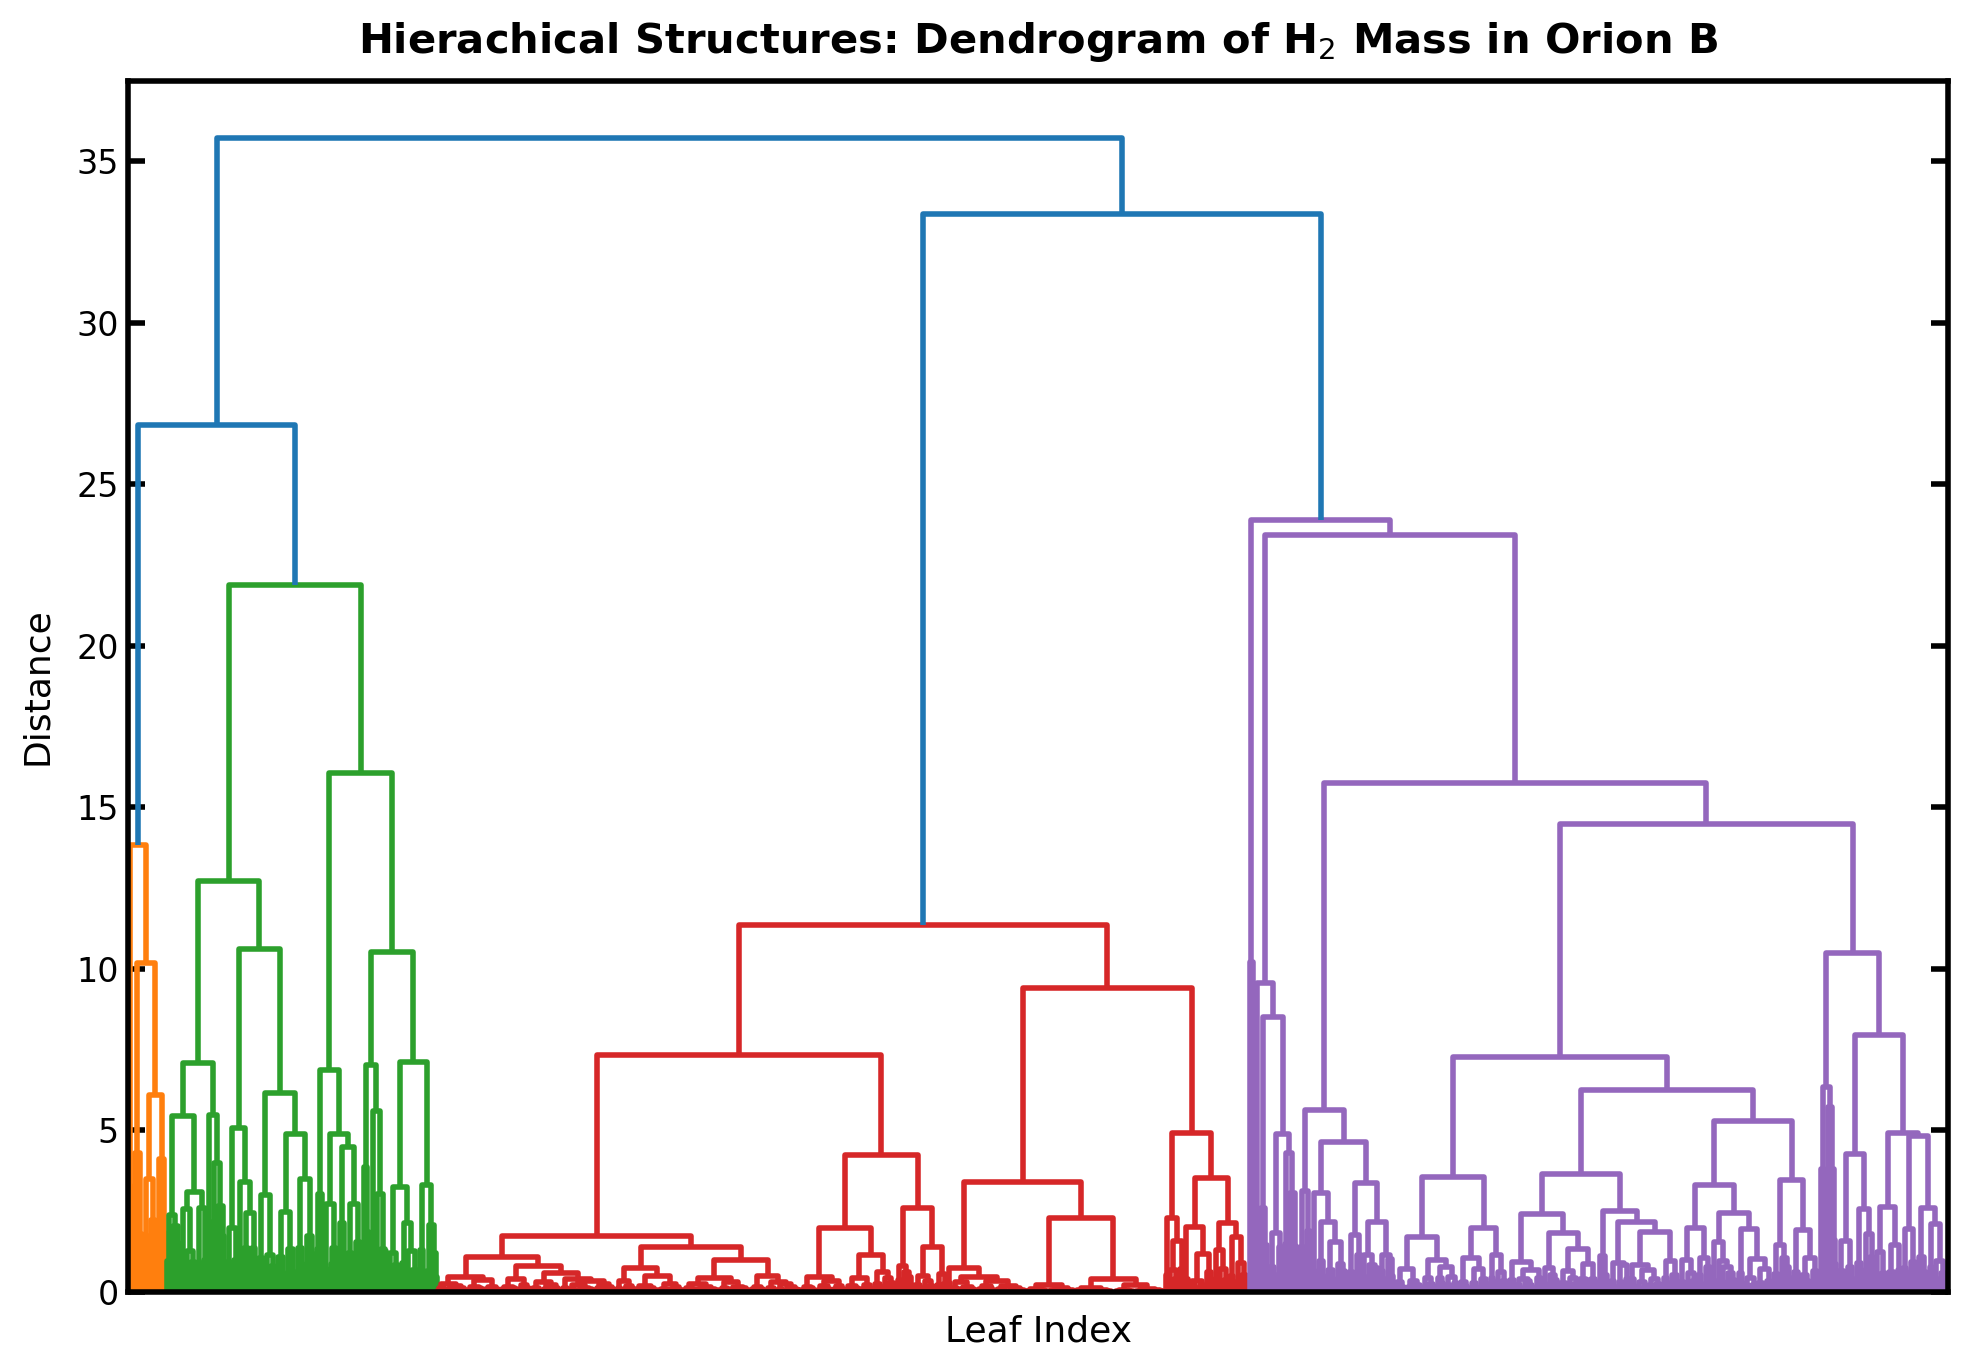
\includegraphics[width=0.5\textwidth]{figures/dendogram_B.png}
    \caption{}
    \label{fig:dendrogram_B}
\end{figure}

\subsection{MSD Plane}

\begin{figure}[t]
    \centering
    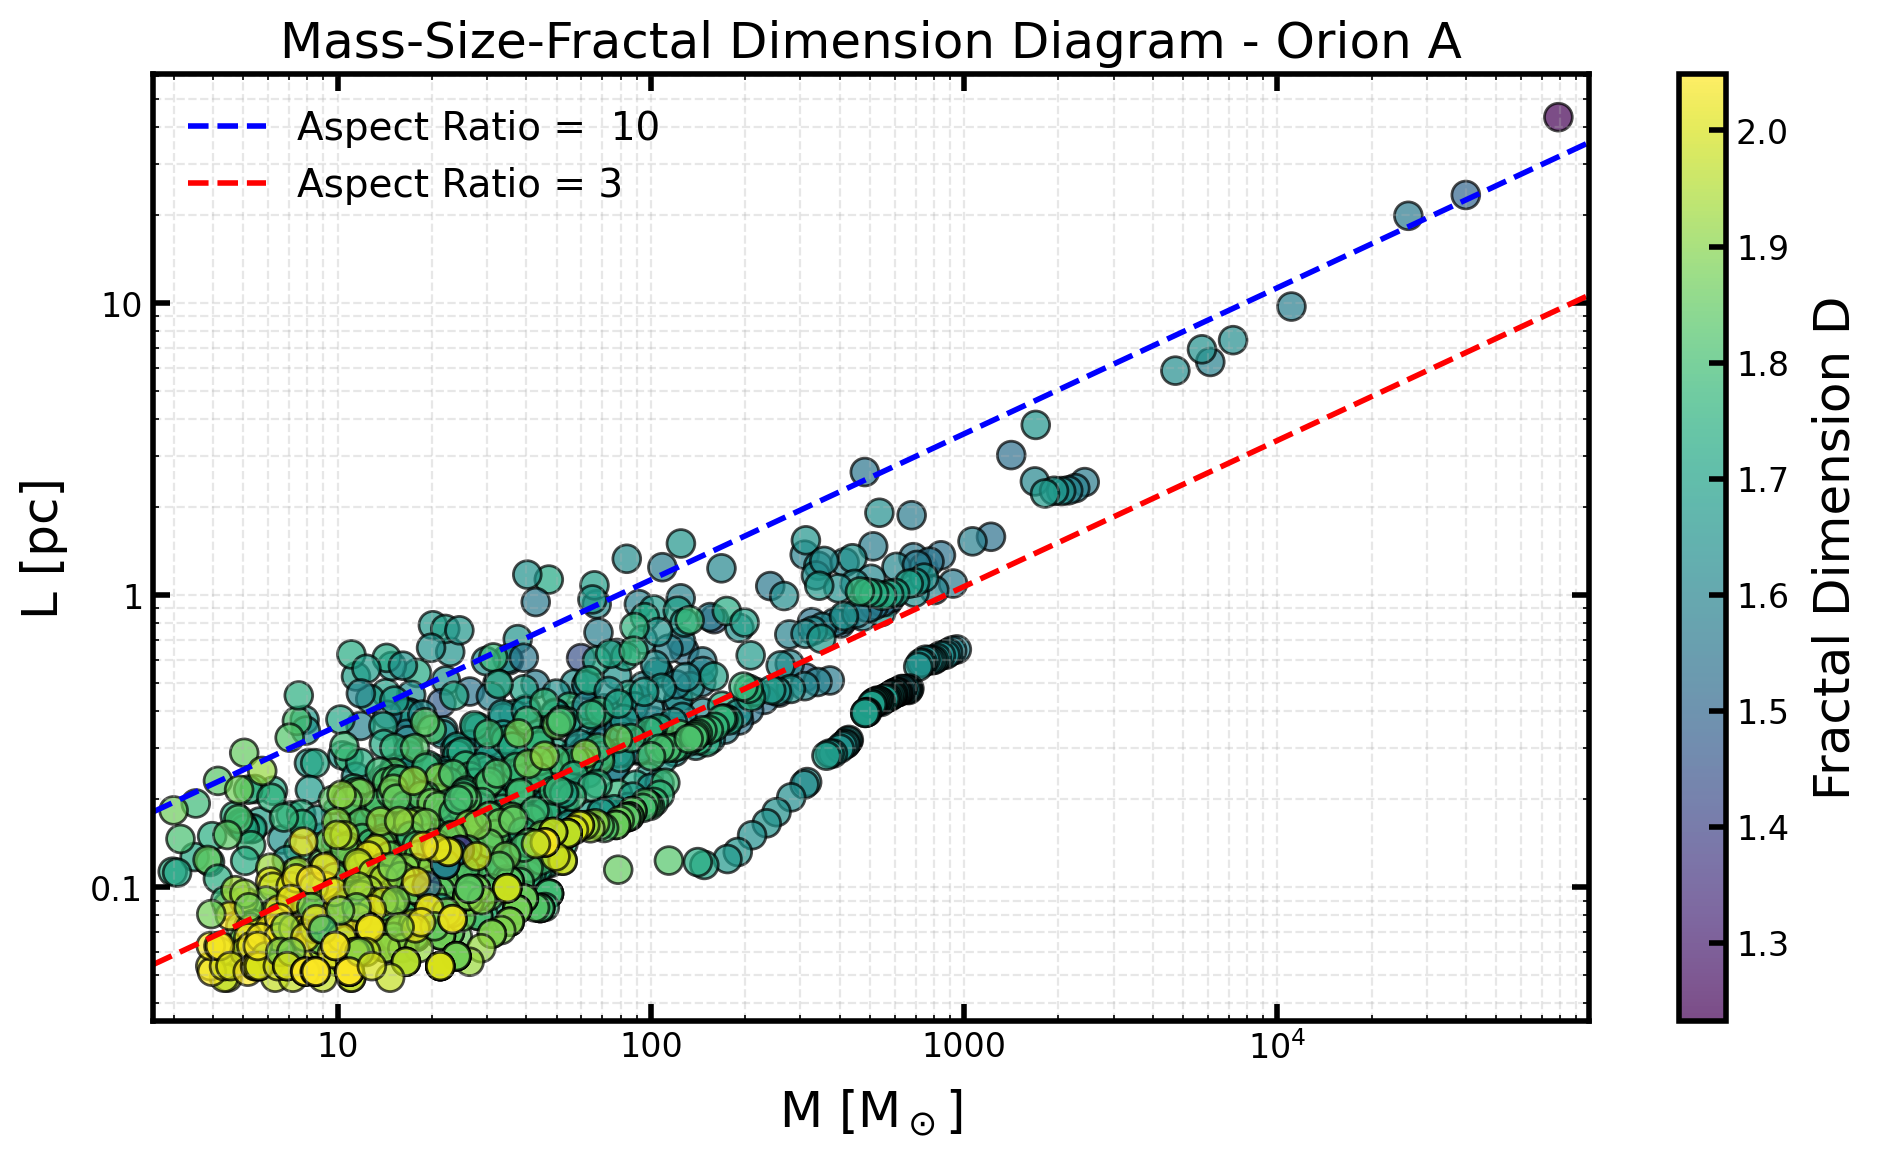
\includegraphics[width=0.5\textwidth]{figures/MSD_Orion_A.png}
    \caption{}
    \label{fig:MSD_orion_A}
\end{figure}

\begin{figure}[t]
    \centering
    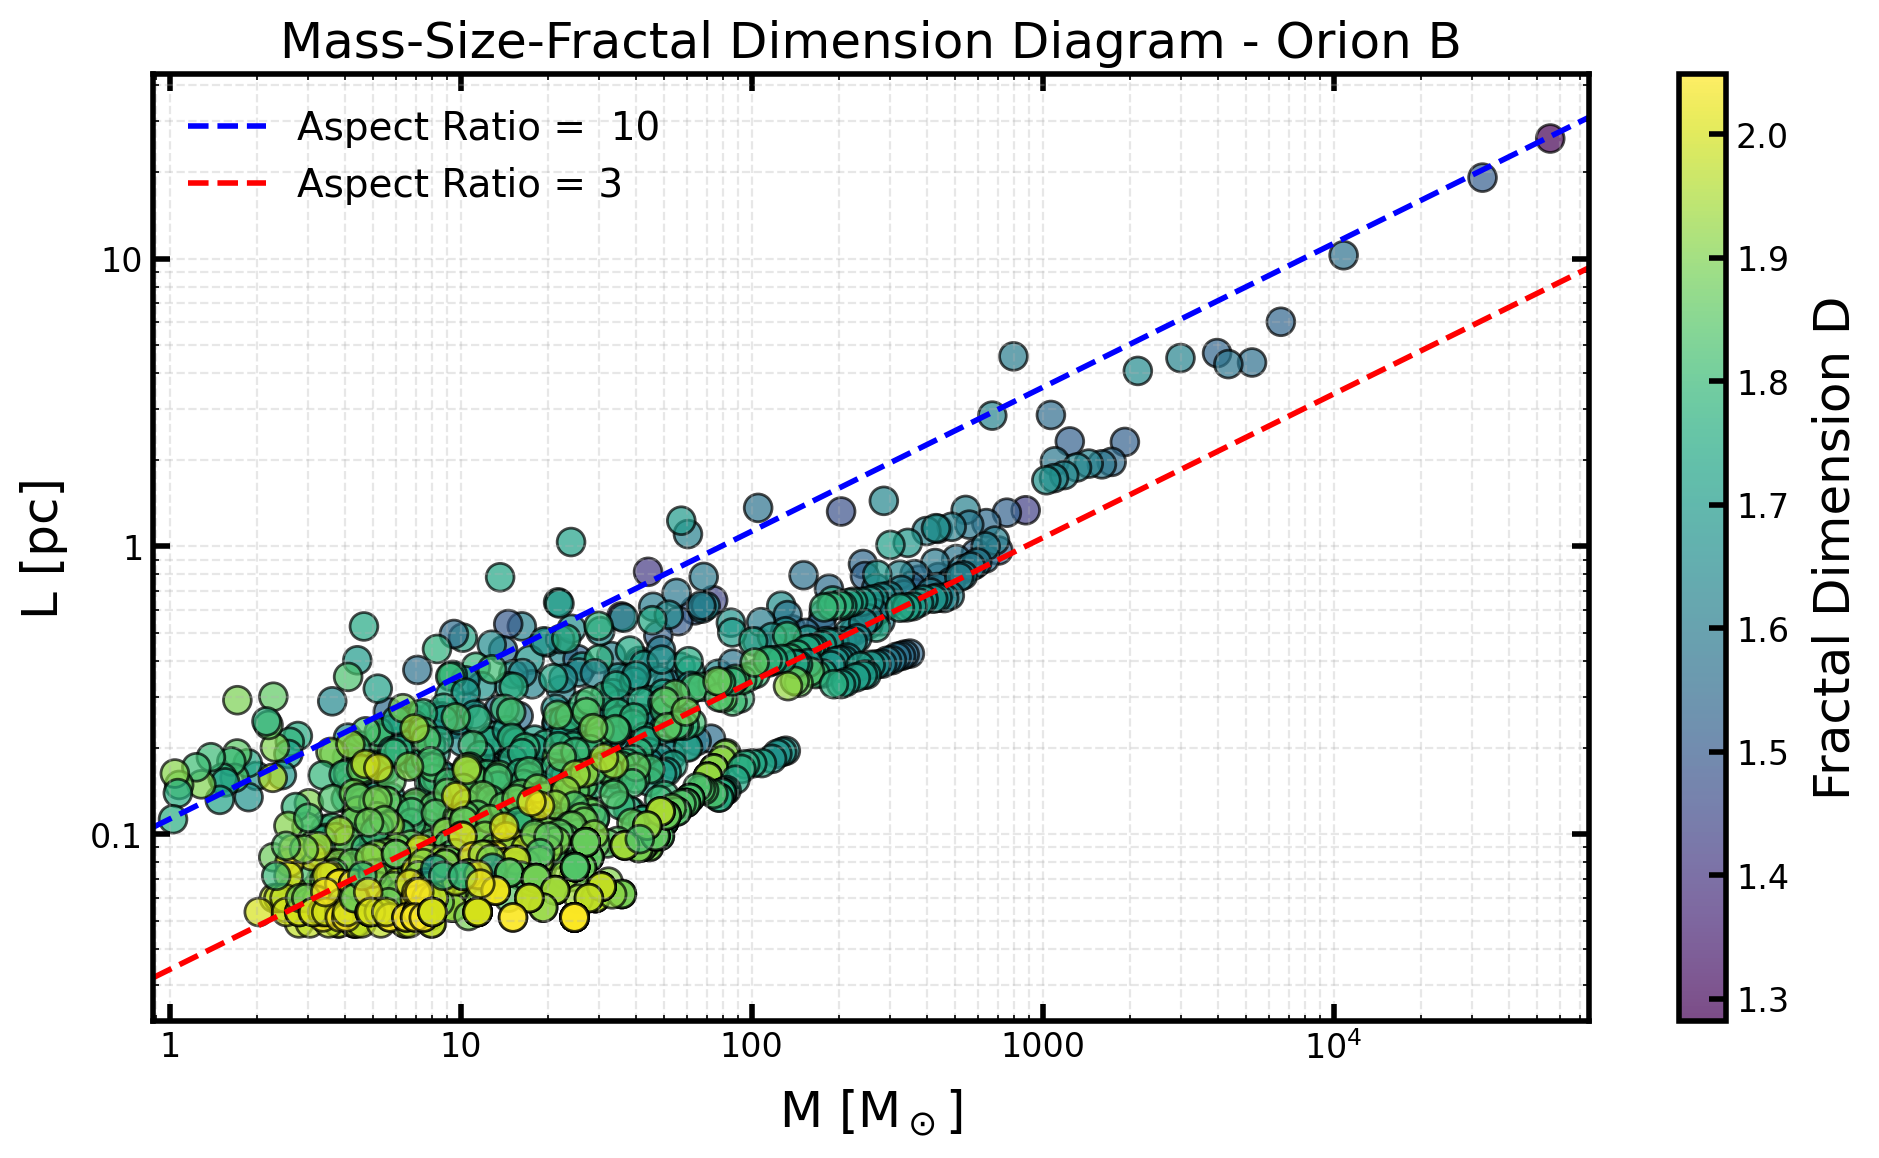
\includegraphics[width=0.5\textwidth]{figures/MSD_Orion_B.png}
    \caption{}
    \label{fig:MSD_orion_B}
\end{figure}

\begin{figure}[t]
    \centering
    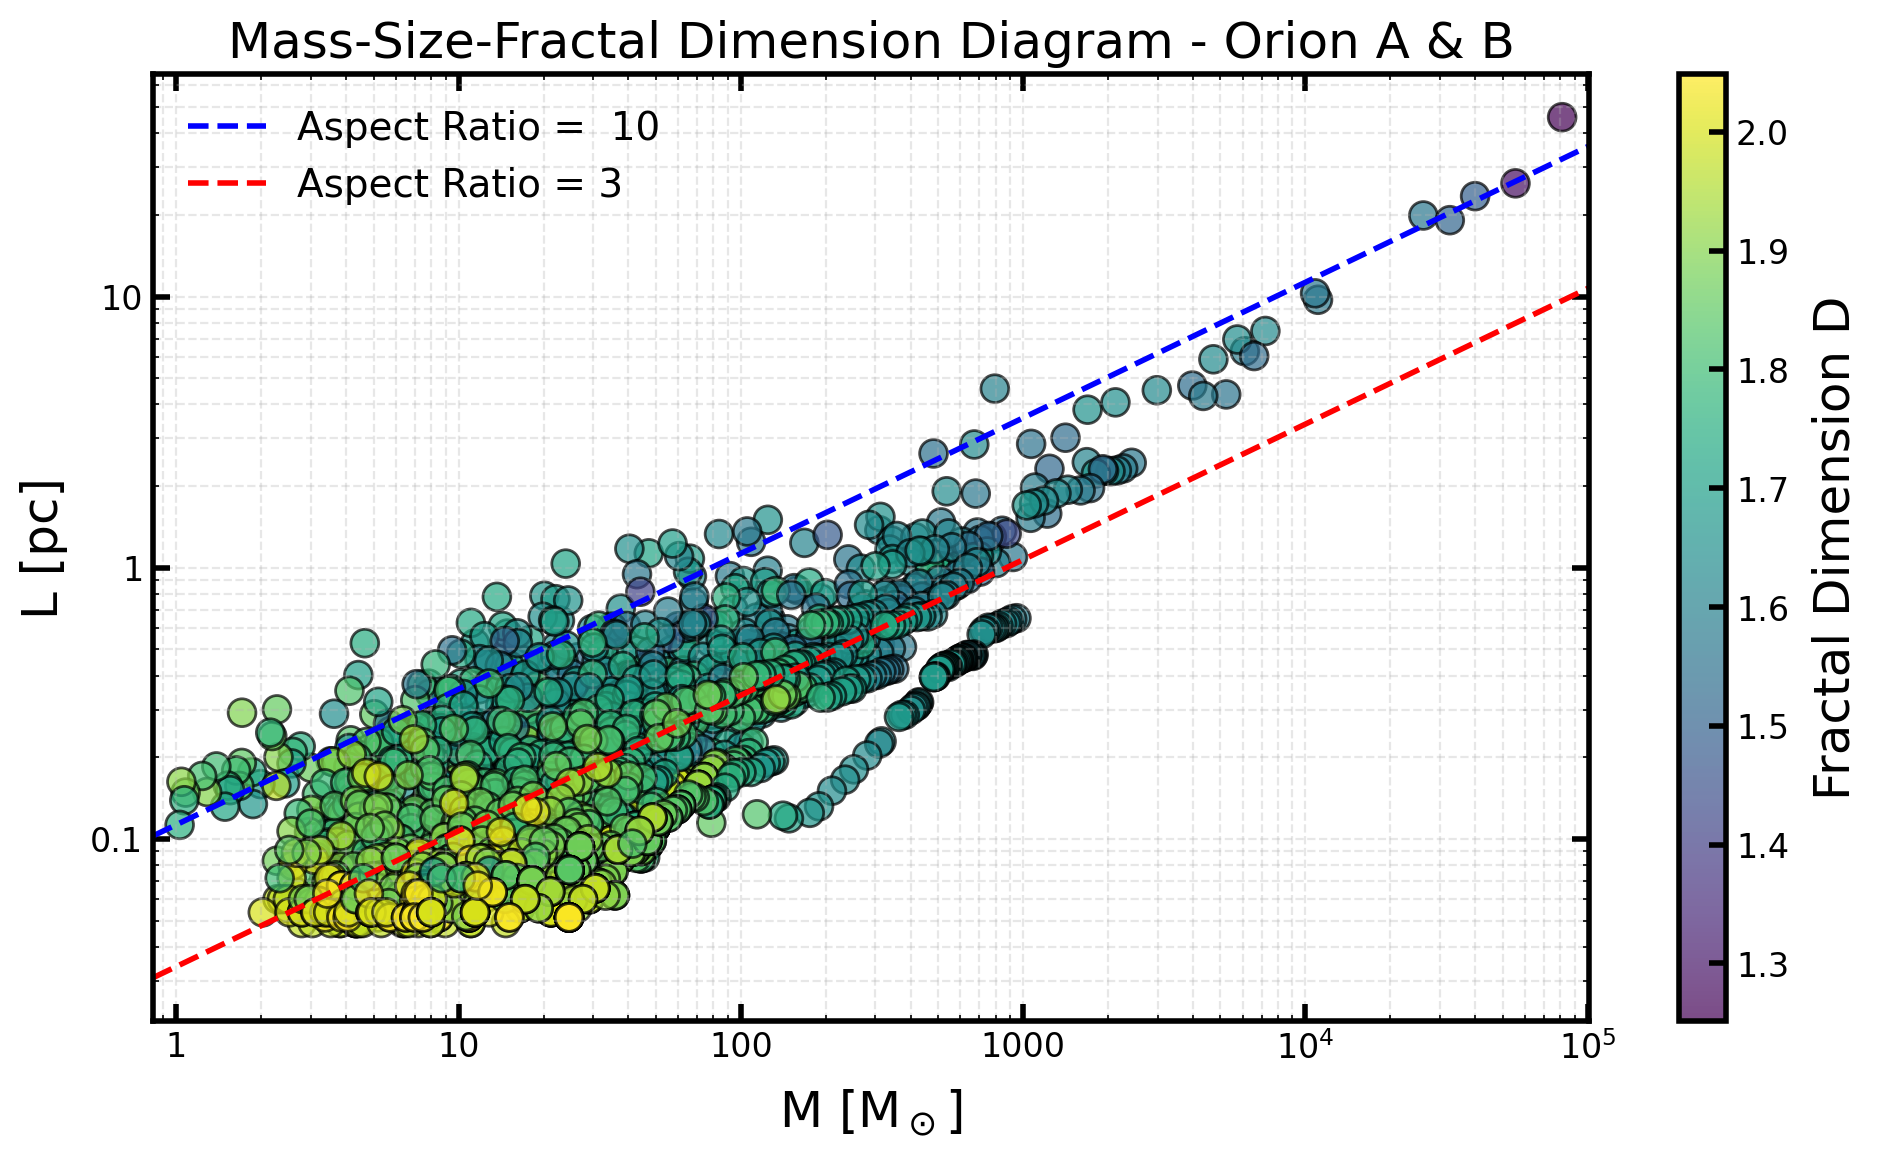
\includegraphics[width=0.5\textwidth]{figures/MSD_Orion_A_B.png}
    \caption{}
    \label{fig:MSD_orion_A_B}
\end{figure}

\subsection{Euler Characteristic}

\section{Star Formation}

